% Important: If latex complains about unicode characters,
% please use "\usepackage[utf8x]{inputenc}" in your preamble
% You can change the size of the picture by putting it into the construct:
% 1) \resizebox{10cm}{!}{"below picture"} to scale horizontally to 10 cm
% 2) \resizebox{!}{15cm}{"below picture"} to scale vertically to 15 cm
% 3) \resizebox{10cm}{15cm}{"below picture"} a combination of above two
% It is not recomended to use the scale option of the tikzpicture environment.
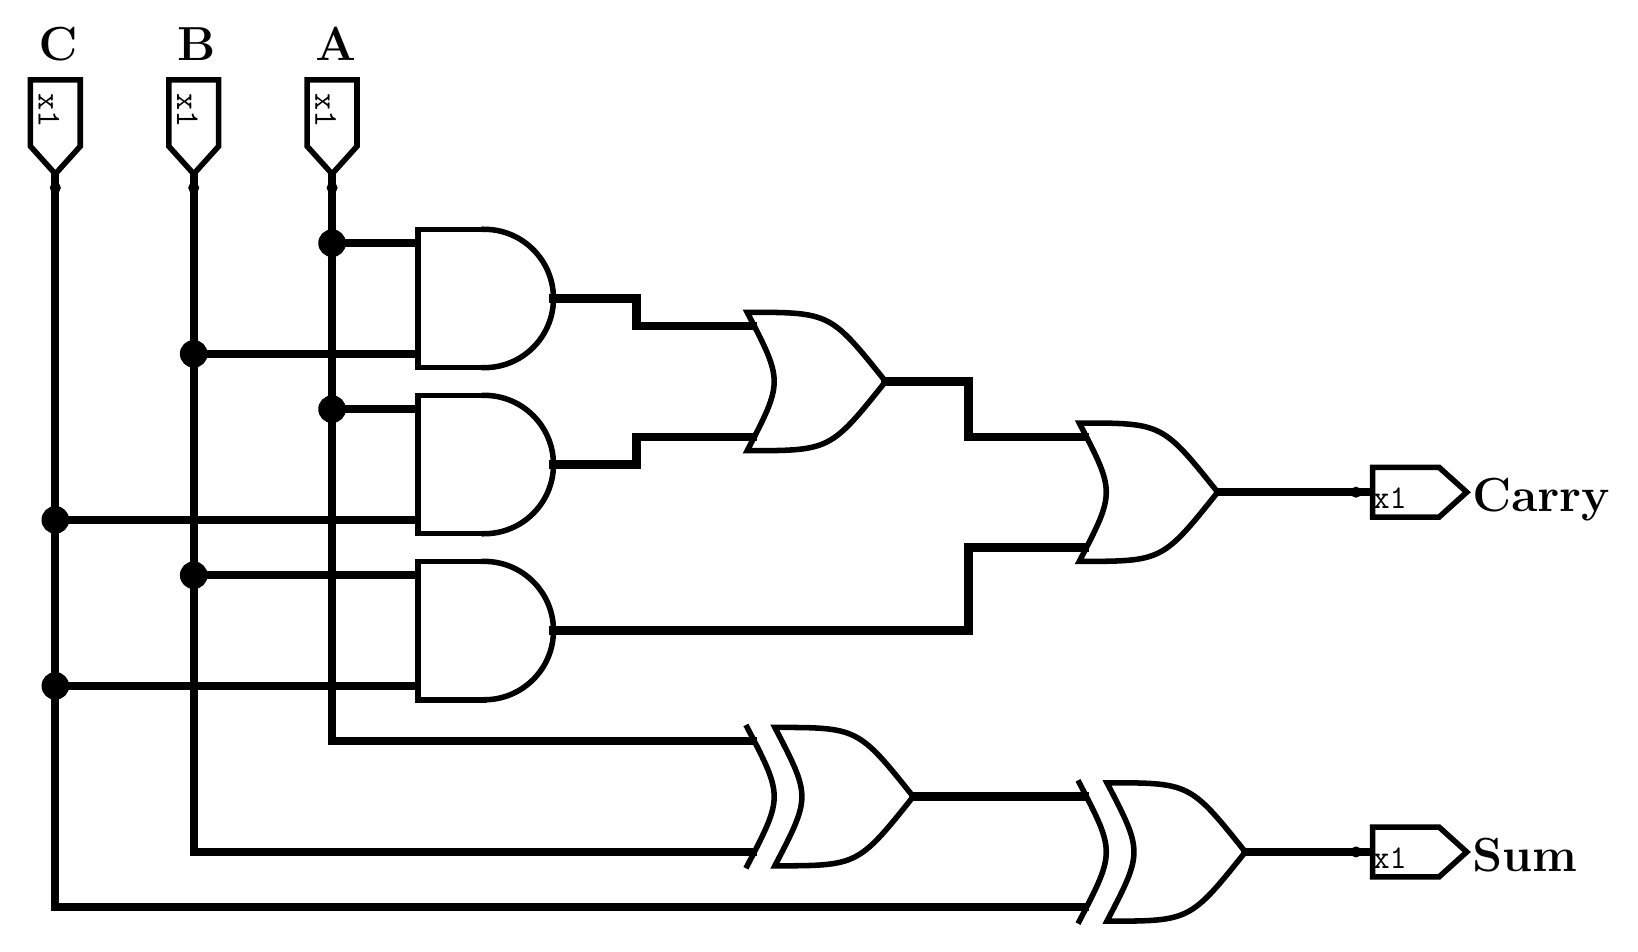
\begin{tikzpicture}[x=1pt,y=-1pt,line cap=rect]
\def\logisimfontA#1{\fontfamily{cmr}{#1}} % Replaced by logisim, original font was "SansSerif"
\def\logisimfontB#1{\fontfamily{cmtt}{#1}} % Replaced by logisim, original font was "Monospaced"
\definecolor{custcol_0_0_0}{RGB}{0, 0, 0}
\definecolor{custcol_ff_ff_ff}{RGB}{255, 255, 255}
\draw [line width=3.0pt, custcol_0_0_0 ]  (435.0,176.0) -- (485.0,176.0) ;
\draw [line width=3.0pt, custcol_0_0_0 ]  (445.0,306.0) -- (485.0,306.0) ;
\draw [line width=3.0pt, custcol_0_0_0 ]  (65.0,206.0) -- (145.0,206.0) ;
\draw [line width=3.0pt, custcol_0_0_0 ]  (115.0,86.0) -- (115.0,146.0) -- (145.0,146.0) ;
\draw [line width=3.0pt, custcol_0_0_0 ]  (15.0,186.0) -- (15.0,246.0) ;
\fill [line width=3.0pt, custcol_0_0_0]  (115.0,146.0) ellipse (5.0 and 5.0 );
\fill [line width=3.0pt, custcol_0_0_0]  (115.0,86.0) ellipse (5.0 and 5.0 );
\fill [line width=3.0pt, custcol_0_0_0]  (15.0,246.0) ellipse (5.0 and 5.0 );
\fill [line width=3.0pt, custcol_0_0_0]  (15.0,186.0) ellipse (5.0 and 5.0 );
\fill [line width=3.0pt, custcol_0_0_0]  (65.0,126.0) ellipse (5.0 and 5.0 );
\fill [line width=3.0pt, custcol_0_0_0]  (65.0,206.0) ellipse (5.0 and 5.0 );
\draw [line width=3.0pt, custcol_0_0_0 ]  (15.0,61.0) -- (15.0,66.0) -- (15.0,186.0) -- (145.0,186.0) ;
\draw [line width=2.0pt, custcol_0_0_0 ]  (6.0,51.0) -- (15.0,61.0) -- (24.0,51.0) -- (24.0,27.0) -- (6.0,27.0) -- cycle;
\logisimfontB{\fontsize{12pt}{12pt}\selectfont\node[inner sep=0, outer sep=0, custcol_0_0_0, anchor=base west, rotate=-90.0] at  (9.0,32.0)  {x1};}
\logisimfontA{\fontsize{16pt}{16pt}\fontseries{bx}\selectfont\node[inner sep=0, outer sep=0, custcol_0_0_0, anchor=base west] at  (9.0,20.0)  {C};}
\fill [line width=2.0pt, custcol_0_0_0]  (15.0,66.0) ellipse (2.0 and 2.0 );
\draw [line width=3.0pt, custcol_0_0_0 ]  (65.0,61.0) -- (65.0,66.0) -- (65.0,126.0) ;
\draw [line width=2.0pt, custcol_0_0_0 ]  (56.0,51.0) -- (65.0,61.0) -- (74.0,51.0) -- (74.0,27.0) -- (56.0,27.0) -- cycle;
\logisimfontB{\fontsize{12pt}{12pt}\selectfont\node[inner sep=0, outer sep=0, custcol_0_0_0, anchor=base west, rotate=-90.0] at  (59.0,32.0)  {x1};}
\logisimfontA{\fontsize{16pt}{16pt}\fontseries{bx}\selectfont\node[inner sep=0, outer sep=0, custcol_0_0_0, anchor=base west] at  (59.0,20.0)  {B};}
\fill [line width=2.0pt, custcol_0_0_0]  (65.0,66.0) ellipse (2.0 and 2.0 );
\draw [line width=3.0pt, custcol_0_0_0 ]  (115.0,61.0) -- (115.0,66.0) -- (115.0,86.0) -- (145.0,86.0) ;
\draw [line width=2.0pt, custcol_0_0_0 ]  (106.0,51.0) -- (115.0,61.0) -- (124.0,51.0) -- (124.0,27.0) -- (106.0,27.0) -- cycle;
\logisimfontB{\fontsize{12pt}{12pt}\selectfont\node[inner sep=0, outer sep=0, custcol_0_0_0, anchor=base west, rotate=-90.0] at  (109.0,32.0)  {x1};}
\logisimfontA{\fontsize{16pt}{16pt}\fontseries{bx}\selectfont\node[inner sep=0, outer sep=0, custcol_0_0_0, anchor=base west] at  (109.0,20.0)  {A};}
\fill [line width=2.0pt, custcol_0_0_0]  (115.0,66.0) ellipse (2.0 and 2.0 );
\draw [line width=2.0pt, custcol_0_0_0] (170.0,131.0) arc (90.0:-90.0:25.0 and 25.0 );
\draw [line width=2.0pt, custcol_0_0_0 ]  (170.0,81.0) -- (146.0,81.0) -- (146.0,131.0) -- (170.0,131.0) ;
\draw [line width=3.0pt, custcol_0_0_0 ]  (195.0,106.0) -- (225.0,106.0) -- (225.0,116.0) -- (265.0,116.0) -- (267.0,116.0) ;
\draw [line width=3.0pt, custcol_0_0_0 ]  (195.0,166.0) -- (225.0,166.0) -- (225.0,156.0) -- (265.0,156.0) -- (267.0,156.0) ;
\draw [line width=2.0pt, custcol_0_0_0 ]  (315.0,136.0) .. controls  (295.0,111.0)  ..  (265.0,111.0) .. controls  (278.0,136.0)  ..  (265.0,161.0) .. controls  (295.0,161.0)  ..  (315.0,136.0) -- cycle ;
\draw [line width=2.0pt, custcol_0_0_0] (170.0,191.0) arc (90.0:-90.0:25.0 and 25.0 );
\draw [line width=2.0pt, custcol_0_0_0 ]  (170.0,141.0) -- (146.0,141.0) -- (146.0,191.0) -- (170.0,191.0) ;
\draw [line width=2.0pt, custcol_0_0_0] (170.0,251.0) arc (90.0:-90.0:25.0 and 25.0 );
\draw [line width=2.0pt, custcol_0_0_0 ]  (170.0,201.0) -- (146.0,201.0) -- (146.0,251.0) -- (170.0,251.0) ;
\draw [line width=3.0pt, custcol_0_0_0 ]  (115.0,146.0) -- (115.0,266.0) -- (265.0,266.0) -- (267.0,266.0) ;
\draw [line width=3.0pt, custcol_0_0_0 ]  (145.0,126.0) -- (65.0,126.0) -- (65.0,206.0) -- (65.0,306.0) -- (265.0,306.0) -- (267.0,306.0) ;
\draw [line width=2.0pt, custcol_0_0_0 ]  (325.0,286.0) .. controls  (305.0,261.0)  ..  (275.0,261.0) .. controls  (288.0,286.0)  ..  (275.0,311.0) .. controls  (305.0,311.0)  ..  (325.0,286.0) -- cycle ;
\draw [line width=2.0pt, custcol_0_0_0 ]  (265.0,261.0) .. controls  (278.0,286.0)  ..  (265.0,311.0) ;
\draw [line width=3.0pt, custcol_0_0_0 ]  (325.0,286.0) -- (385.0,286.0) -- (387.0,286.0) ;
\draw [line width=3.0pt, custcol_0_0_0 ]  (145.0,246.0) -- (15.0,246.0) -- (15.0,326.0) -- (385.0,326.0) -- (387.0,326.0) ;
\draw [line width=2.0pt, custcol_0_0_0 ]  (445.0,306.0) .. controls  (425.0,281.0)  ..  (395.0,281.0) .. controls  (408.0,306.0)  ..  (395.0,331.0) .. controls  (425.0,331.0)  ..  (445.0,306.0) -- cycle ;
\draw [line width=2.0pt, custcol_0_0_0 ]  (385.0,281.0) .. controls  (398.0,306.0)  ..  (385.0,331.0) ;
\draw [line width=3.0pt, custcol_0_0_0 ]  (315.0,136.0) -- (345.0,136.0) -- (345.0,156.0) -- (385.0,156.0) -- (387.0,156.0) ;
\draw [line width=3.0pt, custcol_0_0_0 ]  (195.0,226.0) -- (345.0,226.0) -- (345.0,196.0) -- (385.0,196.0) -- (387.0,196.0) ;
\draw [line width=2.0pt, custcol_0_0_0 ]  (435.0,176.0) .. controls  (415.0,151.0)  ..  (385.0,151.0) .. controls  (398.0,176.0)  ..  (385.0,201.0) .. controls  (415.0,201.0)  ..  (435.0,176.0) -- cycle ;
\draw [line width=3.0pt, custcol_0_0_0 ]  (489.0,176.0) -- (486.0,176.0) ;
\draw [line width=2.0pt, custcol_0_0_0 ]  (515.0,167.0) -- (525.0,176.0) -- (515.0,185.0) -- (491.0,185.0) -- (491.0,167.0) -- cycle;
\logisimfontB{\fontsize{12pt}{12pt}\selectfont\node[inner sep=0, outer sep=0, custcol_0_0_0, anchor=base west] at  (491.0,182.0)  {x1};}
\logisimfontA{\fontsize{16pt}{16pt}\fontseries{bx}\selectfont\node[inner sep=0, outer sep=0, custcol_0_0_0, anchor=base west] at  (527.0,183.0)  {Carry};}
\fill [line width=2.0pt, custcol_0_0_0]  (485.0,176.0) ellipse (2.0 and 2.0 );
\draw [line width=3.0pt, custcol_0_0_0 ]  (489.0,306.0) -- (486.0,306.0) ;
\draw [line width=2.0pt, custcol_0_0_0 ]  (515.0,297.0) -- (525.0,306.0) -- (515.0,315.0) -- (491.0,315.0) -- (491.0,297.0) -- cycle;
\logisimfontB{\fontsize{12pt}{12pt}\selectfont\node[inner sep=0, outer sep=0, custcol_0_0_0, anchor=base west] at  (491.0,312.0)  {x1};}
\logisimfontA{\fontsize{16pt}{16pt}\fontseries{bx}\selectfont\node[inner sep=0, outer sep=0, custcol_0_0_0, anchor=base west] at  (527.0,313.0)  {Sum};}
\fill [line width=2.0pt, custcol_0_0_0]  (485.0,306.0) ellipse (2.0 and 2.0 );
\end{tikzpicture}

